\section{ProtoDUNE-ND}
\label{sec:protodune-nd}
In this section, the technical design of the proposed ProtoDUNE-ND at Fermilab is described. First, a consideration of the available neutrino beamlines at Fermilab is carried out in Section~\ref{sec:neutrino-flux}, which shows that the on-axis medium-energy NuMI beam provides a rate closest to that of the future, intense, LBNF beamline~\cite{DUNE3, dune_opt_flux}, making the MINOS-ND hall the ideal location for this prototype. %Second, a discussion of the MINOS-ND hall is provided in Section~\ref{sec:minos-hall}, with consideration given to the existing and required infrastructure to support the ProtoDUNE-ND detectors.
Then, a discussion of the technical aspects of the ProtoDUNE-ND detector design is given: a description of the ArgonCube 2x2 Demonstrator module is given in Section~\ref{sec:2x2-design}, and a description of potential downstream tracking detectors is given in Section~\ref{sec:tracking_detectors}. %\todo{Modify as appropriate... if there's only ArgonCube information available, we can note the possibility of others being included, and comment on the branch points when decisions about whether to include them or not must be made.}

\subsection{Neutrino flux study}
\label{sec:neutrino-flux}
The LBNF beamline is an intense source of muon (anti-)neutrinos, with a much higher flux of neutrinos than accelerator neutrino beams currently in operation~\cite{DUNE3,dune_opt_flux}. A key design requirement for the DUNE near detectors, and one of the primary concerns motivating this ProtoDUNE-ND proposal, is how well the near detector components will perform in a high multiplicity environment. It is therefore worth asking how suitable existing beamlines are for providing a useful neutrino beam test for the proposed near detector components.

\begin{figure}[htb]
  \centering
  \subfloat[Flux\label{subfig:flux}]    {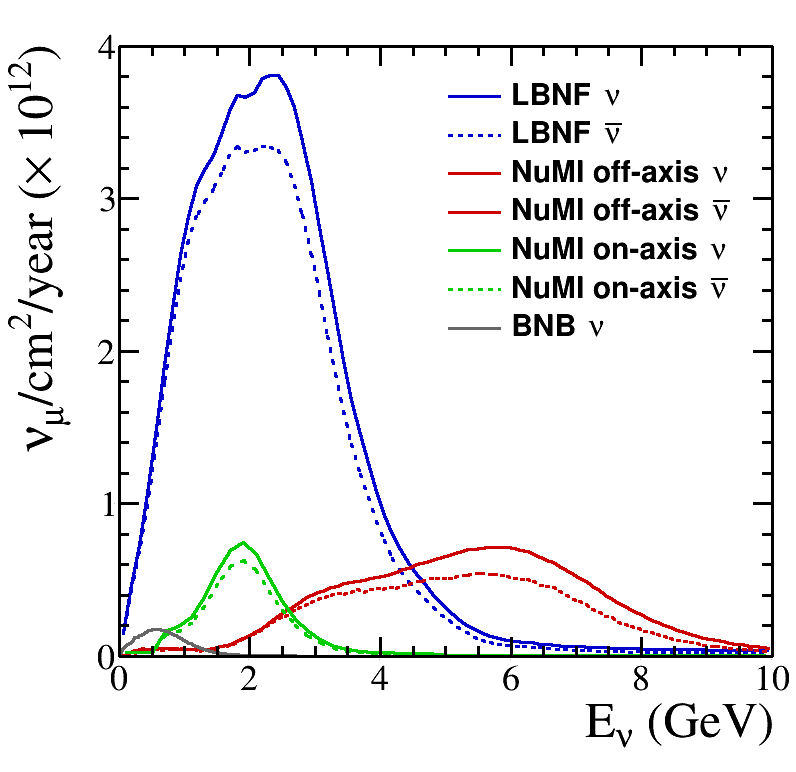
\includegraphics[width=0.5\textwidth]{plots/fnal_flux_comparison.png}}
  \subfloat[Rate\label{subfig:rate}]    {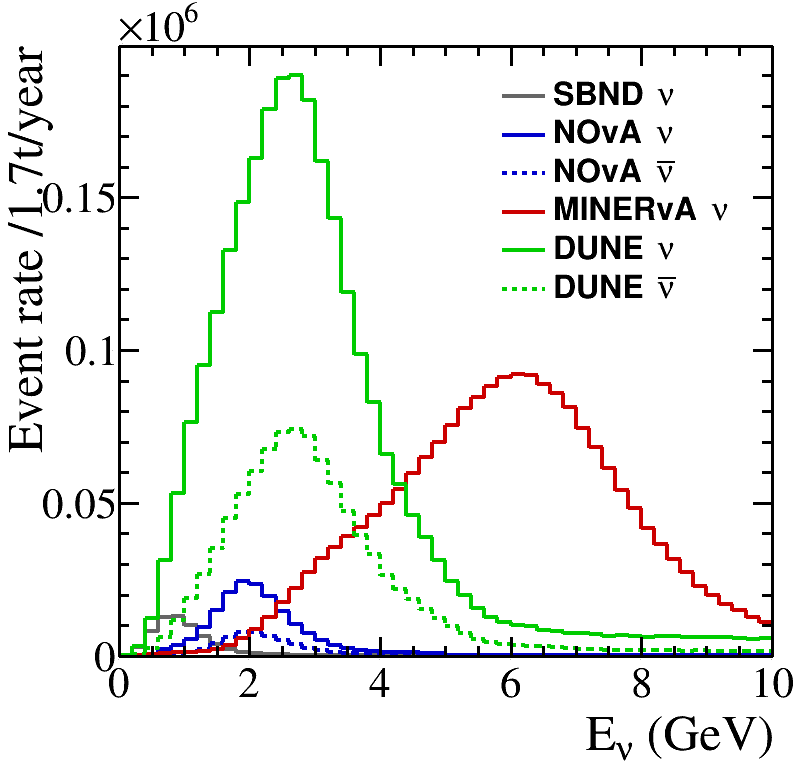
\includegraphics[width=0.5\textwidth]{plots/2x2_Enu_all.png}}
  \caption{Comparison of the absolutely normalized fluxes for different neutrino beamlines at Fermilab, and the expected yearly rates in the ArgonCube 2x2 Demonstrator module's 1.7t active LAr volume as a function of \enu, produced using GENIE v2.12.10 with the ``ValenciaQEBergerSehgalCOHRES'' configuration~\cite{genie}.}
  \label{fig:beam_options}
\end{figure}

In Figure~\ref{subfig:flux}, the currently available neutrino fluxes at various near detector halls in Fermilab are compared, on an absolutely normalized scale, to the LBNF three-horn optimized flux at the \SI{574}{\metre} near detector site~\cite{dune_opt_flux}. The currently available neutrino fluxes considered are the on- and \SI{14}{\milli\radian} off-axis medium-energy neutrinos from the main injector (NuMI) beam~\cite{numi}, which corresponds to the MINOS and NOvA near detector halls; and the booster neutrino beam (BNB) at the SBND hall~\cite{Antonello:2015lea}. The FY2017 delivered protons on target (POT) was used to produce a yearly flux and rate for the BNB ($3.3\times 10^{20}$) and NuMI ($5.06\times 10^{20}$) beams~\cite{fnal_beam_2017}, and the nominal POT of $1.1 \times 10^{21}$/year was used for the LBNF flux. It is clear that the proposed LBNF flux is significantly more intense than the fluxes sampled at any existing experimental hall. However, due to the roughly linear relationship between neutrino energy and cross section, the measured rate from the on-axis NuMI beam in the MINOS-ND hall is approximately the same as for the planned LBNF flux, and is therefore the most desirable currently functional experimental hall at Fermilab in which to situate ProtoDUNE-ND. The rate has been produced with the GENIE neutrino interaction Monte Carlo package~\cite{genie}, using v2.12.10 with the ValenciaQEBergerSehgalCOHRES configuration. Note that the rate is normalized to the active volume of the ArgonCube 2x2 Demonstrator module, showing that significant statistics will be accumulated in a matter of months of ProtoDUNE-ND operation.

\FloatBarrier
%\subsection{MINOS near detector hall}
%\label{sec:minos-hall}
%\begin{itemize}
%\item Size of the hall
%\item Existing infrastructure required for the test
%\item Need to consider whether we need to move anything (e.g. MINERvA) to make space
%\item New infrastructure to be put in for the test --> Barry Norris/ Alan Bross. Probably need to discuss language with Steve Brice to make it forceful enough
%\end{itemize}

\subsection{ArgonCube 2x2 Demonstrator module}
\label{sec:2x2-design}

ArgonCube, and the ArgonCube 2x2 Demonstrator module are described in Ref.~\cite{argoncube_loi}. However, a number of significant improvements to the design have been made since then, to account for the advancements made in the ArgonCube R\&D program. In particular, the four modules of the ArgonCube 2x2 Demonstrator module will not test separate technologies, as design choices have already been informed by smaller scale tests. Instead, the modules will be functionally identical, to allow for more sophisticated reconstruction tests. Of course, with ProtoDUNE-ND in place, it would be possible to modify aspects of the modules, or test alternative designs if the ProtoDUNE-ND data motivates further modifications.

\begin{figure}[htbp]
\centering
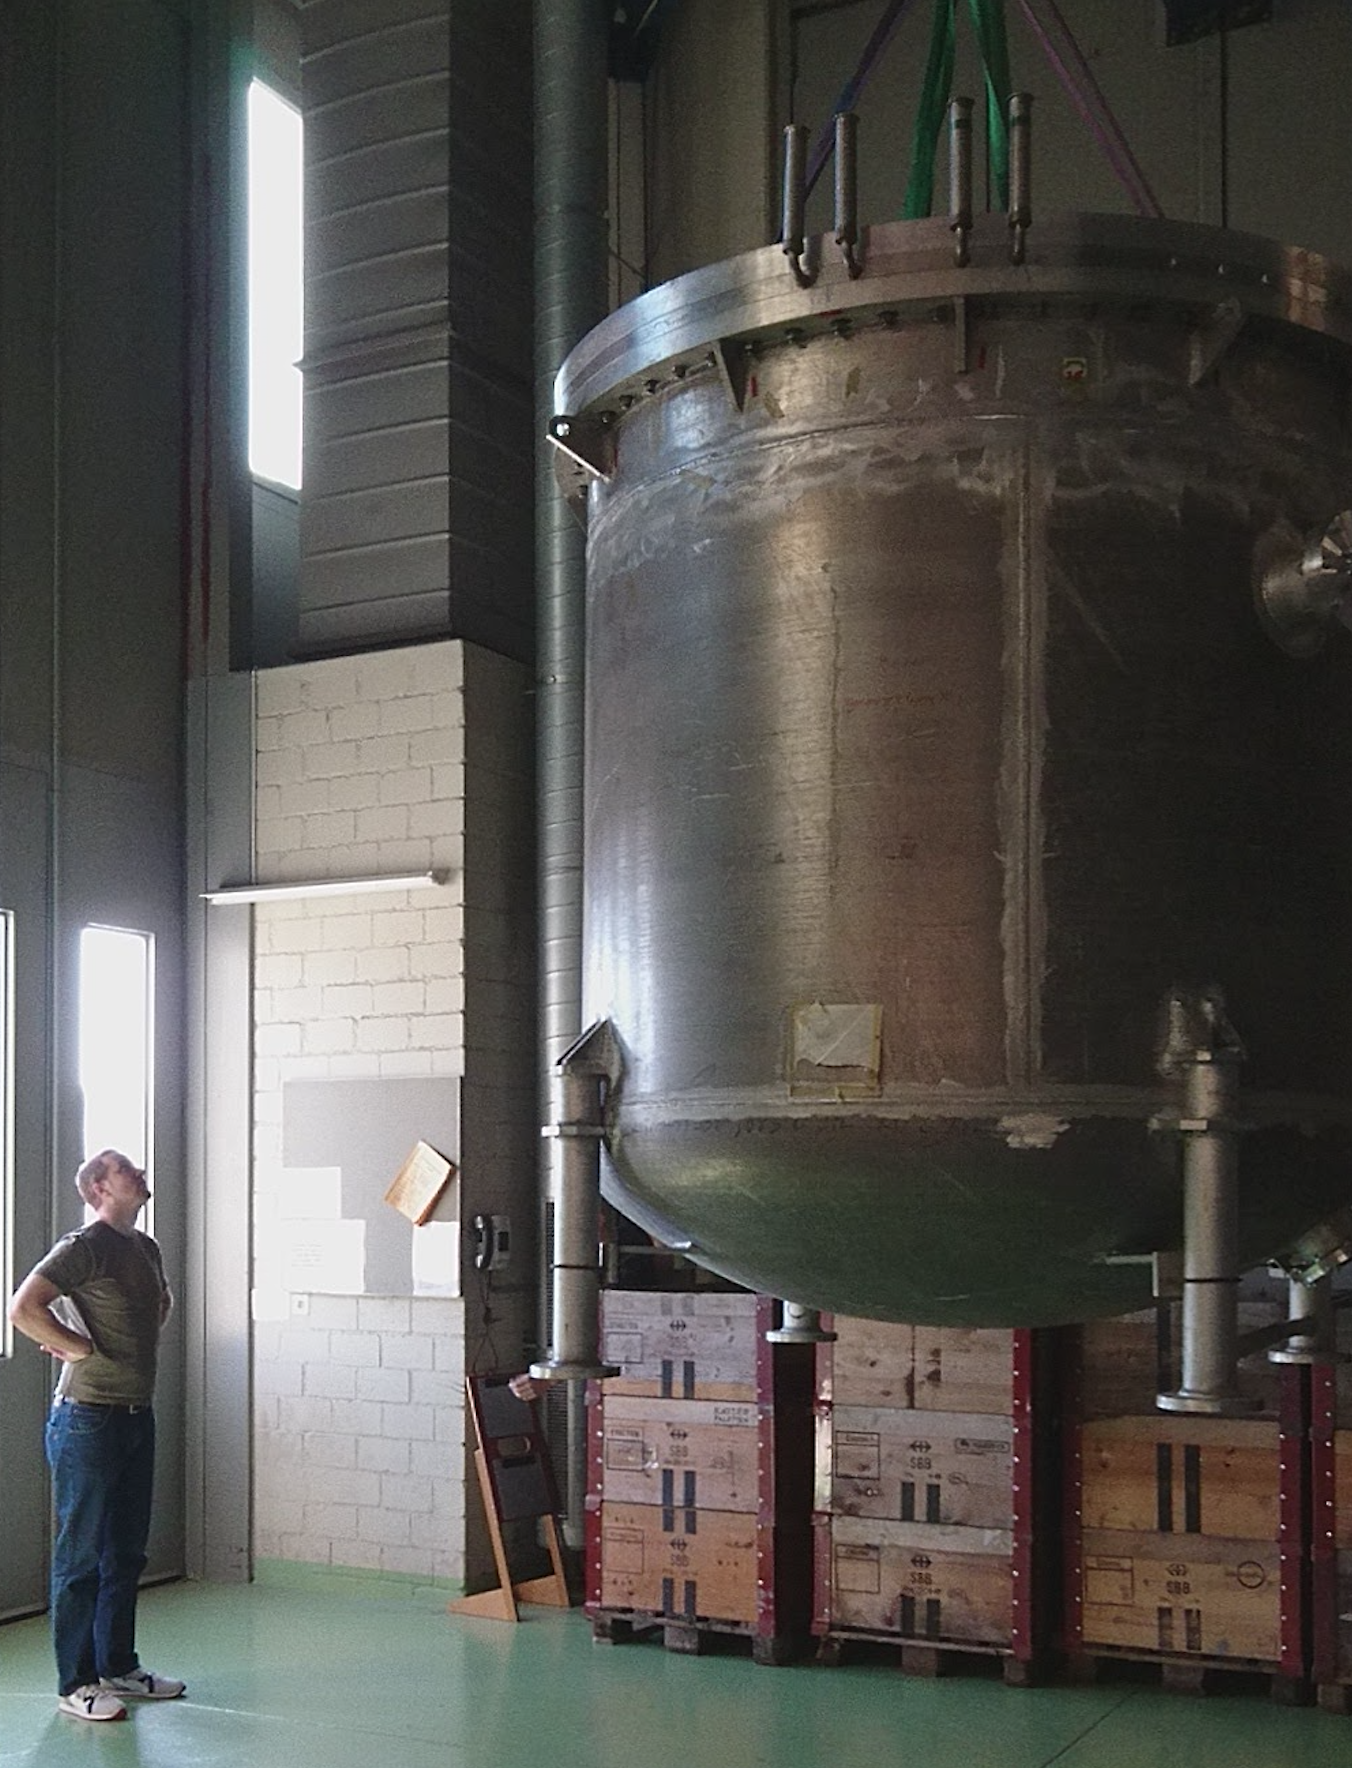
\includegraphics[width=0.45\linewidth]{plots/cryostat}
\caption{The liquid nitrogen-cooled and vacuum-insulated cryostat that will host the ArgonCube 2x2 Demonstrator module, reproduced from Ref.~\cite{argoncube_loi}.}
\label{fig:2x2_cryostat}
\end{figure}

The basic principle of ArgonCube is a detector made of self-contained TPC modules sharing a common cryostat. Each module is made of a rectangular box with a square footprint and a height to be optimized in order to meet the physics goals and/or sensitivity constraints. The ArgonCube 2x2 Demonstrator module will be housed within an existing liquid nitrogen (LN2)-cooled and vacuum-insulated cryostat, shown in Figure~\ref{fig:2x2_cryostat}, which is $\sim$\SI{2.2}{\metre} in diameter, and $\sim$\SI{2.8}{\metre} deep, for a total volume of $\sim$\SI{6}{\metre\cubed}. The size of the cryostat sets the dimensions of the modules for the demonstrator. The square base of each module will be \SI{0.67 x 0.67}{\metre}, and the height will be \SI{1.81}{\metre}. This makes the modules comparable in size to, but slightly smaller than, the proposed ArgonCube DUNE near detector modules, which will have a base of \SI{1 x 1}{\metre}, with a \SI{3.5}{\metre} height; optimized in order to meet the physics goals and sensitivity requirements.

\begin{figure}[htbp]
\centering
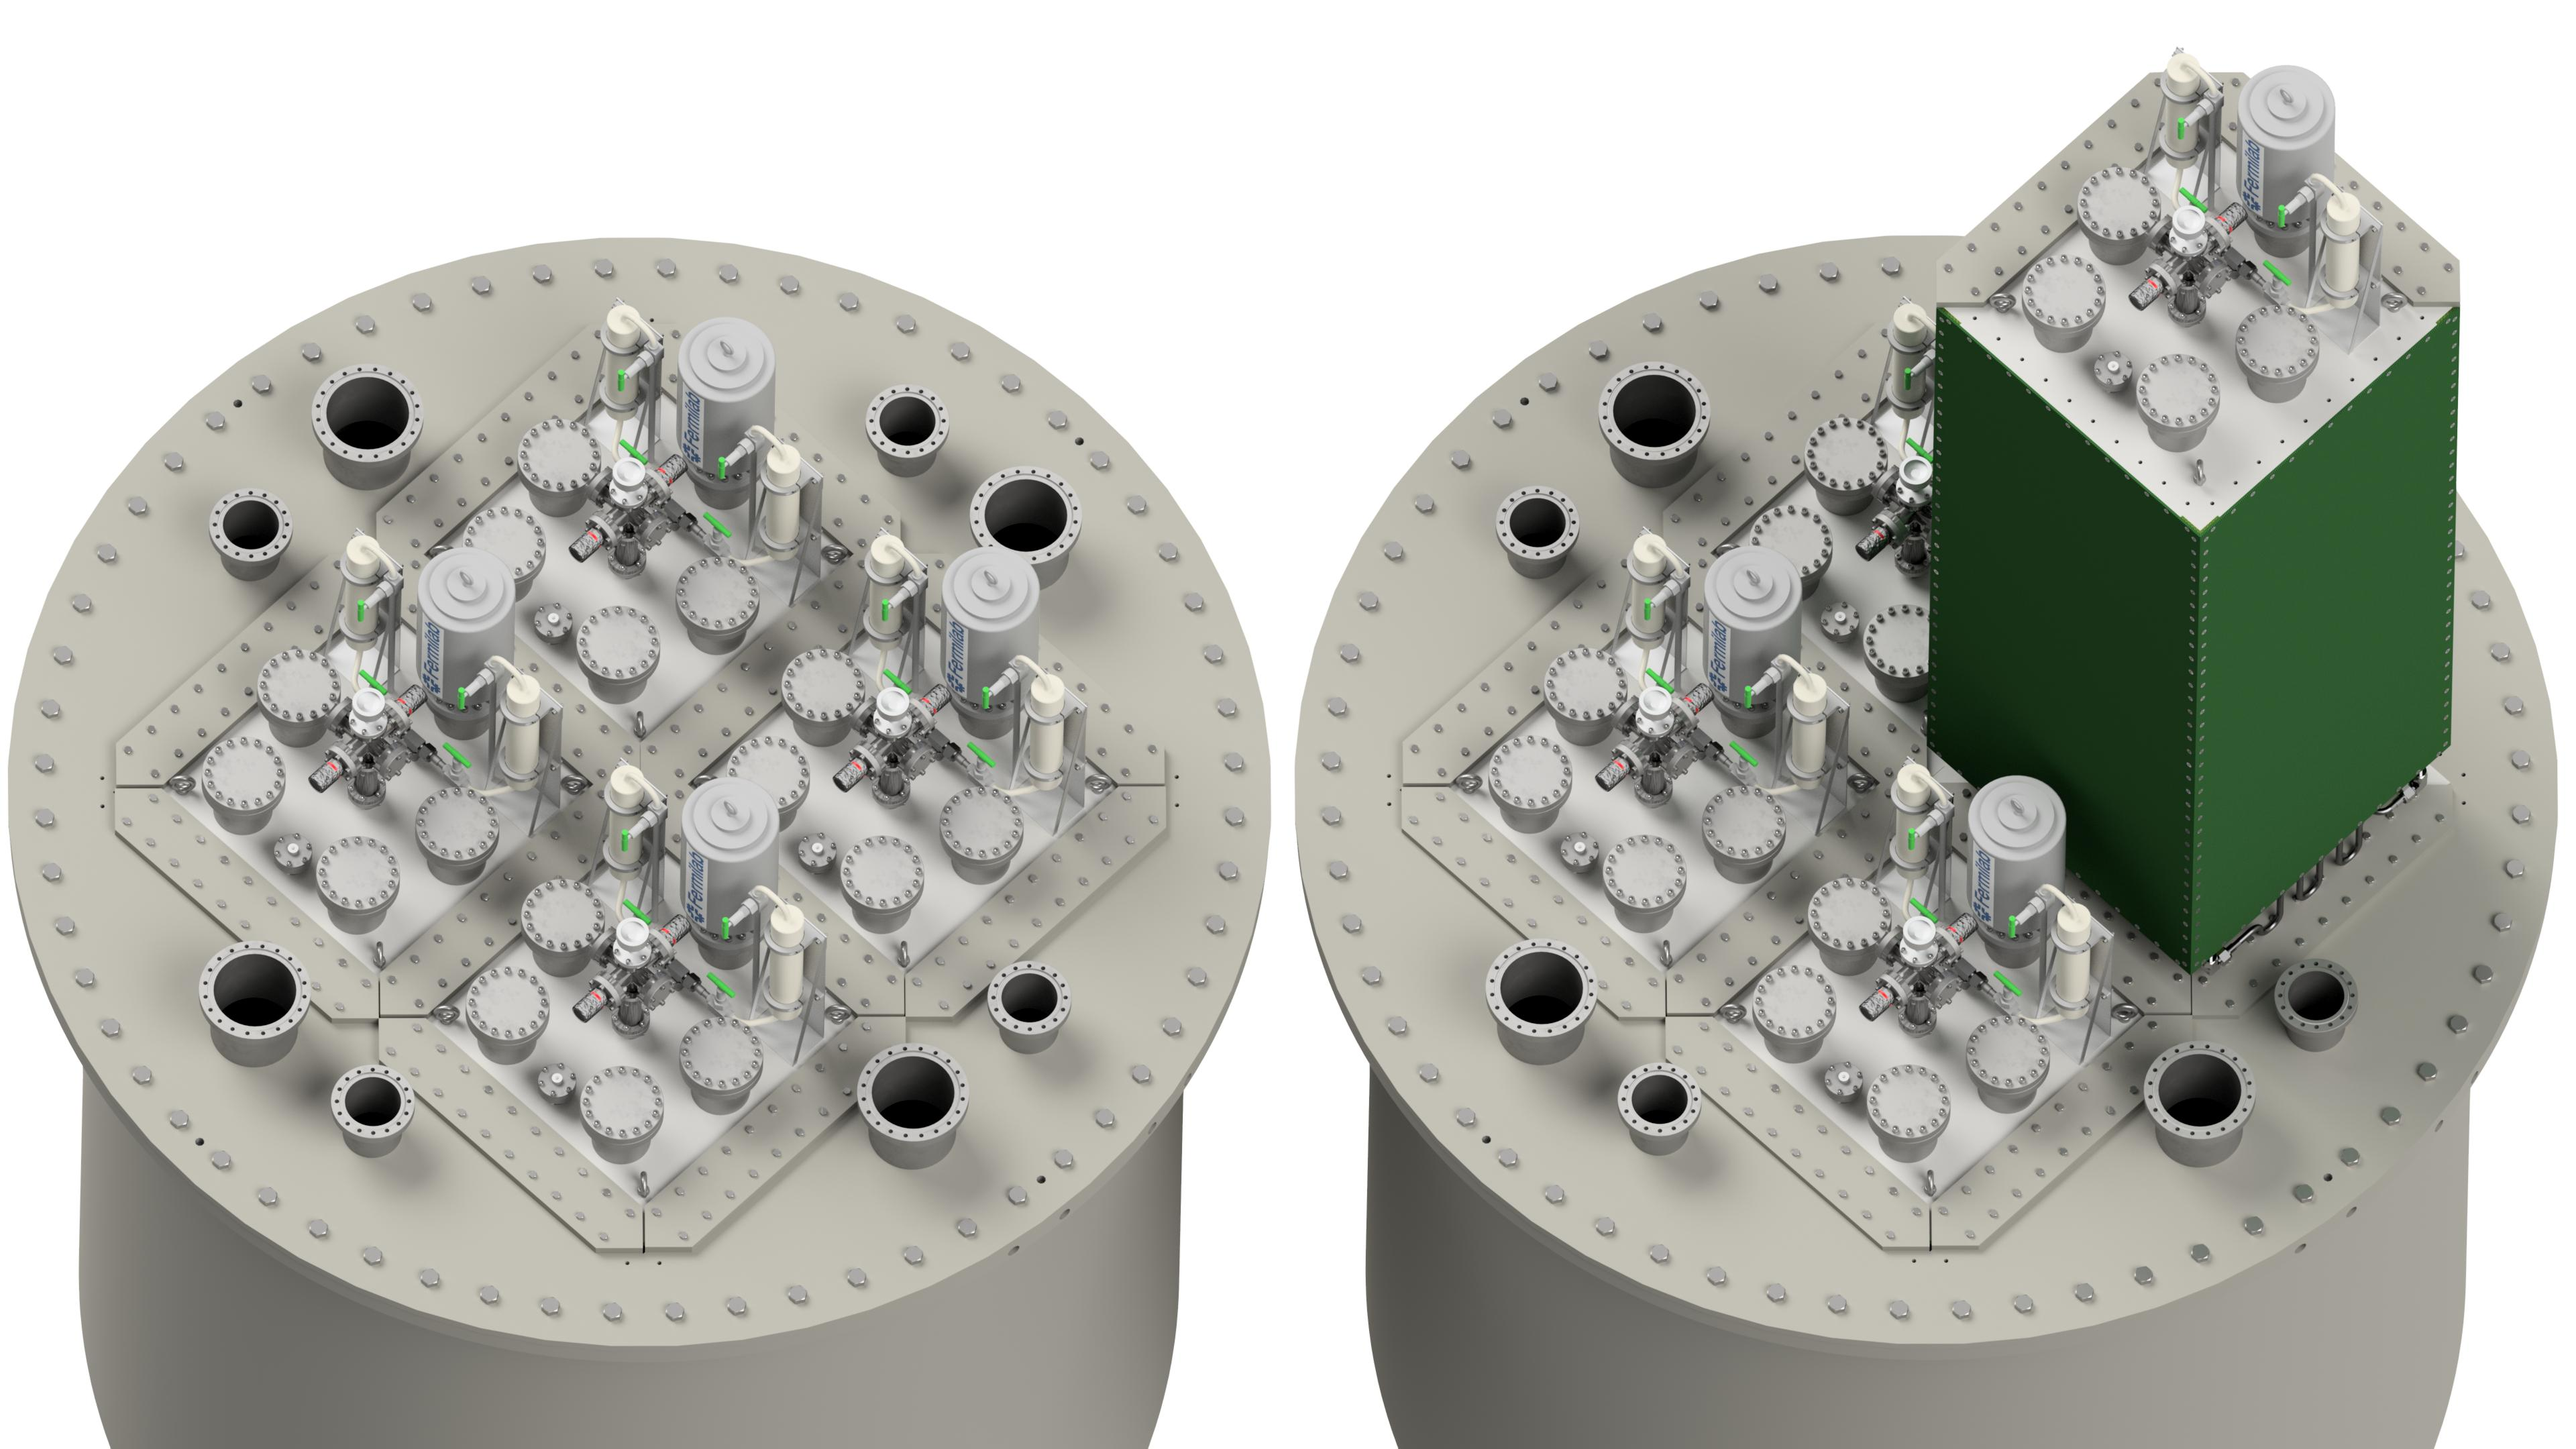
\includegraphics[width=\textwidth]{plots/BathAndModule}
\caption{Illustration of the ArgonCube 2x2 Demonstrator module. The four modules are visible, with one of them is partly extracted, on the right. This figure has been reproduced from Ref.~\cite{argoncube_loi}.}
\label{fig:2x2_extraction}
\end{figure}

Individual modules can be extracted or reinserted into a common LAr bath as needed, as is illustrated in Figure~\ref{fig:2x2_extraction}. This feature will be demonstrated during a commissioning run at Bern, but is not intended to be part of the detector engineering studies in the MINOS-ND hall. Pressure inside the modules is kept close to the bath pressure putting almost no hydrostatic force on the module walls, which allows them to be thin, minimizing the quantity of inactive material in the walls. The purity of the LAr is maintained within the modules, independent of the bath, as will be described below. The argon surrounding the modules needs not meet as stringent purity requirements as the argon inside. Under normal operation conditions all modules are inserted with only clearance distances of \SI{1.5}{\milli\metre} between modules. Cooling power to the bath is supplied by LN2 circulated through lines on the outer surface of the inner cryostat vessel.

\begin{figure}[tbp]
  \centering
  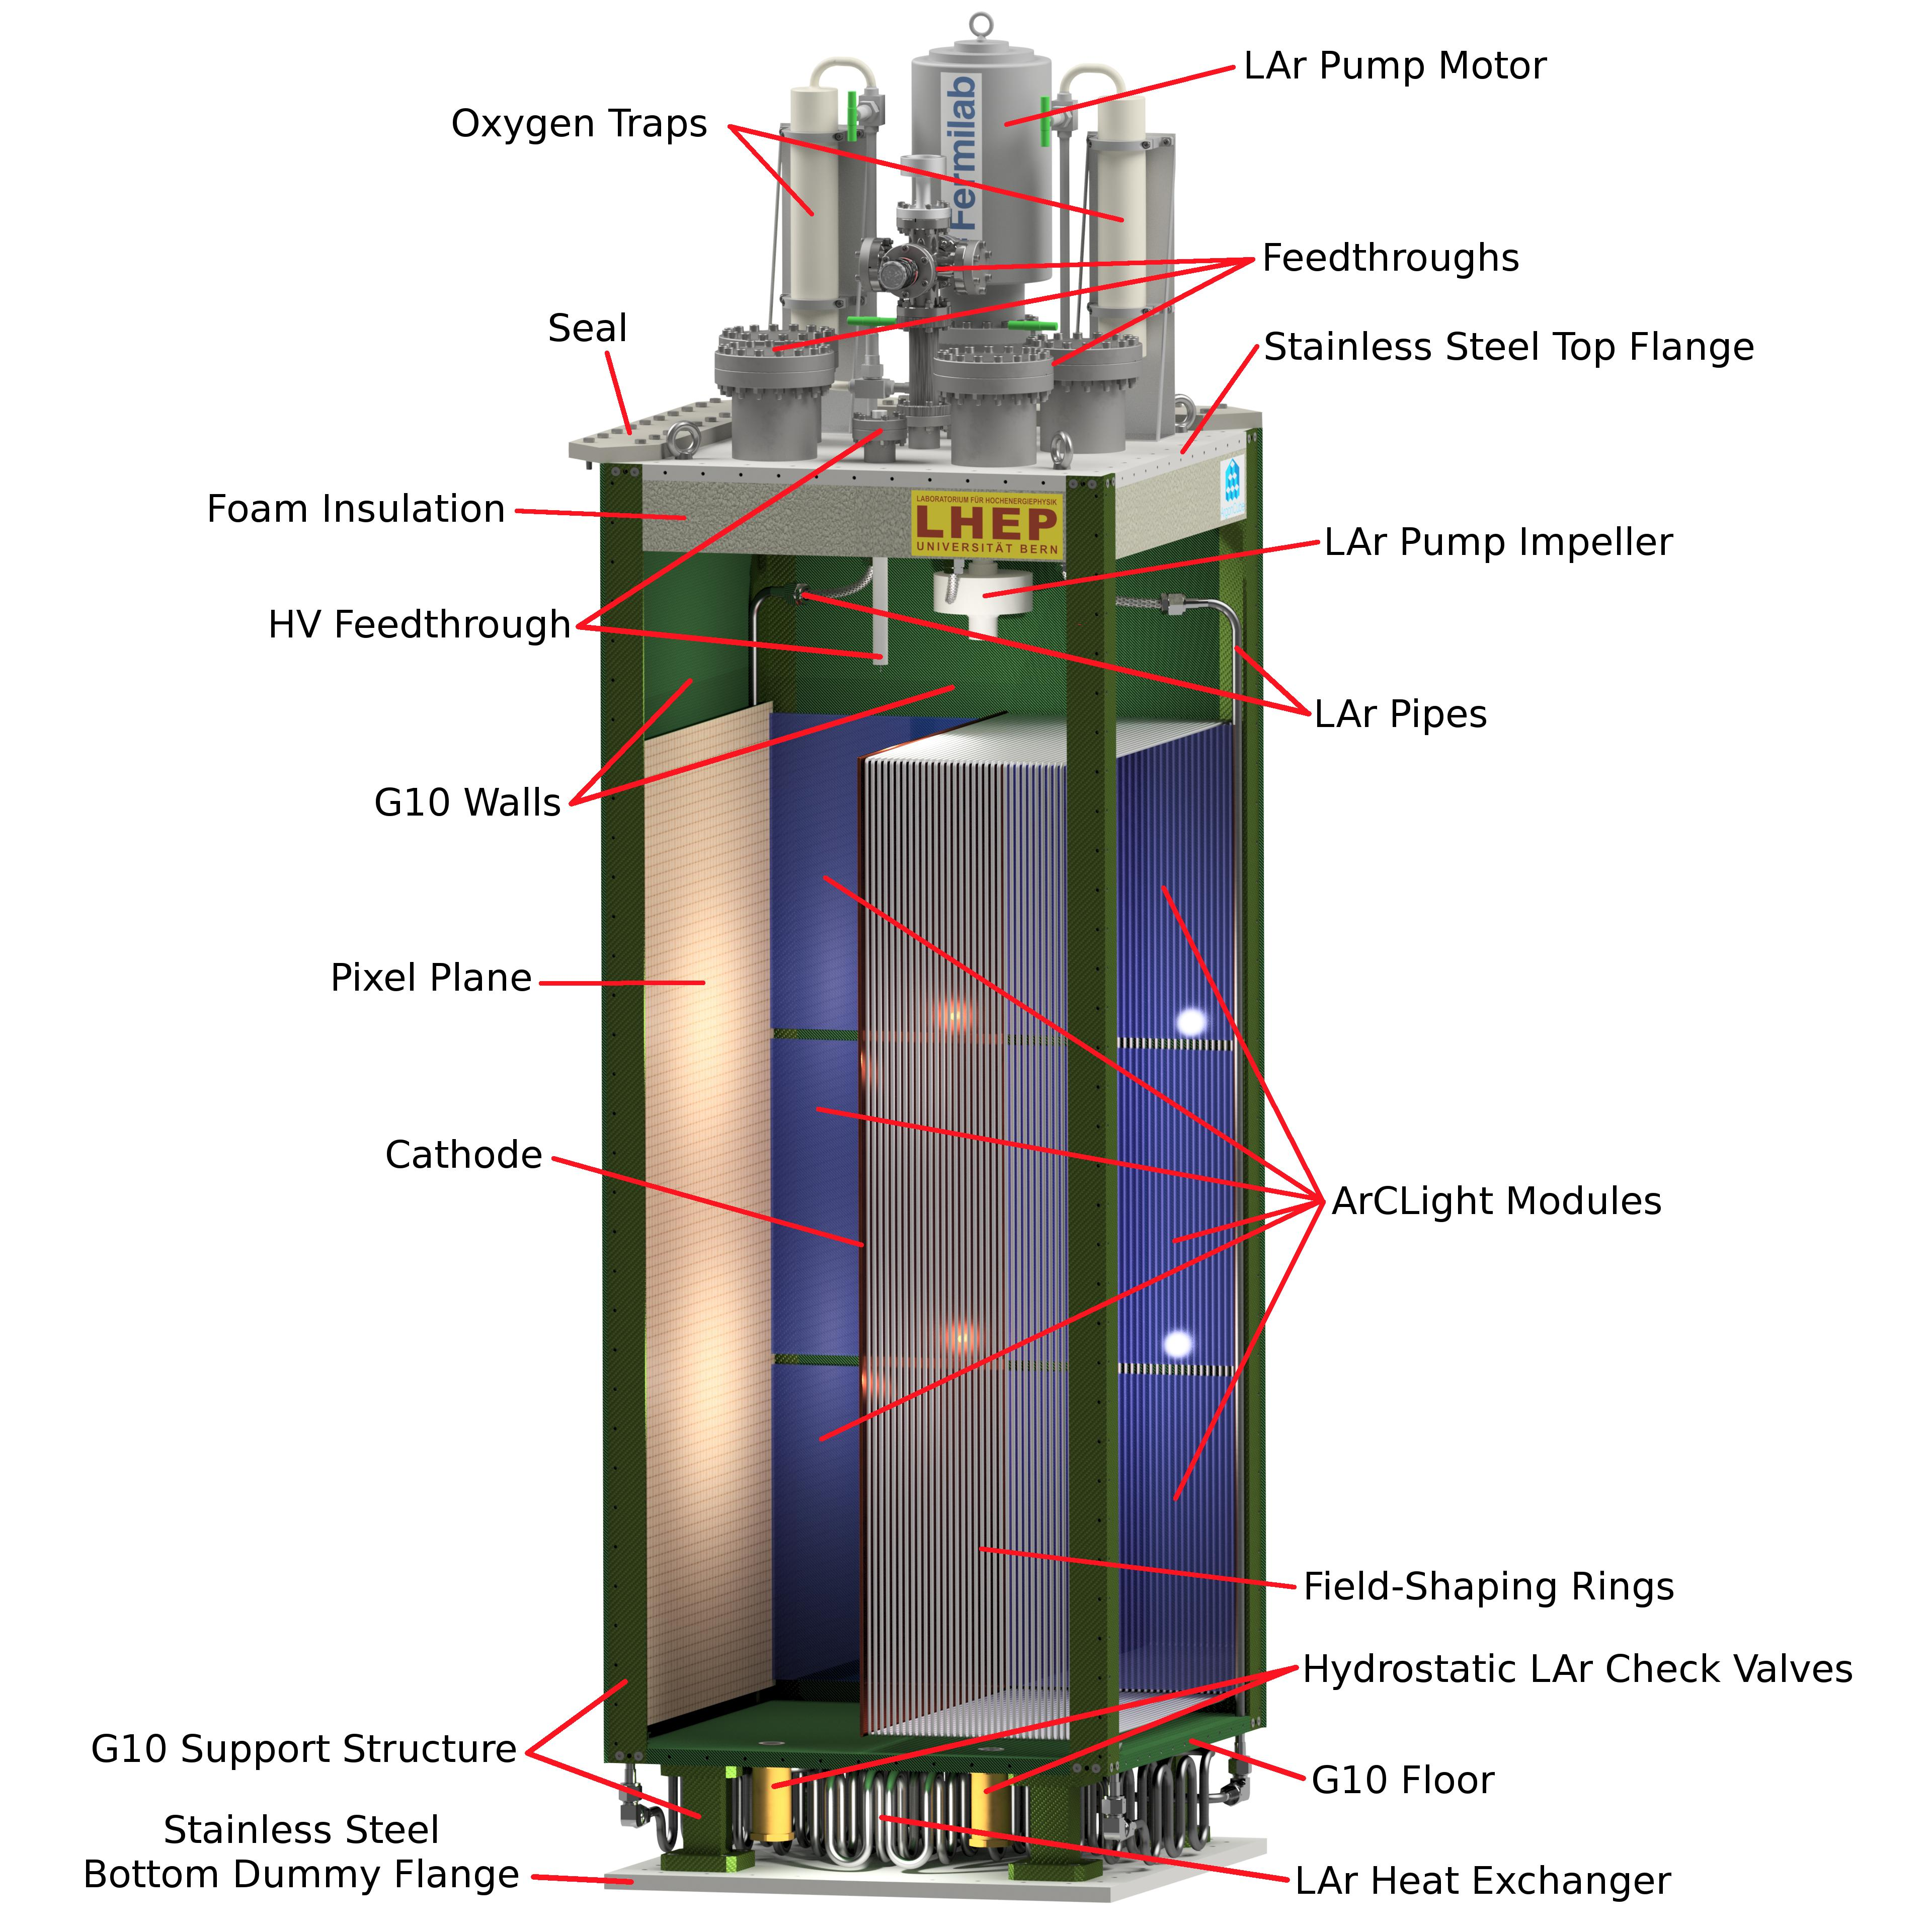
\includegraphics[width=0.8\textwidth]{plots/Normal-Module-4K_labelled}
  \caption[ArgonCube module engineering drawing]{Cutaway drawing of a \SI{0.67 x 0.67 x 1.81}{\metre} ArgonCube module for the 2x2 Demonstrator module. For illustrative purposes the drawing shows traditional field shaping rings instead of a resistive field shell. Note, G10 walls will completely seal the module, isolating it from the neighbouring modules and the outer liquid argon bath.It is also worth noting that the 2x2 will not have individual pumps and filters.}
  \label{fig:ac_module}
\end{figure}

A cutaway drawing of an individual 2x2 module is shown in Figure~\ref{fig:ac_module}. The side walls of each module are made from \SI{1}{\centi\metre} G10 sheets, to which the resistive field shell is laminated. G10's electromagnetic radiation length ($X_{\mathrm{0}} = \SI{19.4}{\centi\metre}$) and hadronic interaction length ($\lambda_{\mathrm{int}} = \SI{53.1}{\centi\metre}$)~\cite{pdg_g10} are both comparable to LAr (14.0~cm and 83.7~cm respectively), making G10 structures in LAr almost transparent for passing particles, allowing for a performance comparable to a monolithic detector. G10 provides a strong dielectric, capable of \SI{200}{\kilo\volt\per\centi\metre} at \SI{1}{\centi\metre} thick~\cite{G10Breakdown}. This dielectric shielding eliminates the need for a clearance volume between the TPCs and the cryostat, while also shielding the TPC from field breakdowns in a neighbouring module. 

The module is split into two TPCs by a central cathode made of an additional resistive layer on a G10 substrate. The segmented drift length does not require a high cathode voltage, and minimizes stored energy. For the 2x2 module footprint of \SI{0.67 x 0.67}{\metre} and an electric field of \SI{1}{\kilo\volt\per\centi\metre} a cathode potential of only \SI{33}{\kilo\volt} is required. Operating a LArTPC at this voltage is feasible without a prohibitive loss of active volume~\cite{argontube}.

The detector is oriented such that the cathodes are parallel to the beam. This minimizes the load on the readout electronics by spreading the event over more channels and reducing the required digitization rate for hit channels. In turn, this reduces the heat load generated at the charge readout and prevents localized boiling.

During filling and emptying of the cryostat, the argon flow is controlled by hydrostatic check valves located at the lower flange of the module, which require a minimal differential pressure of \SI{15}{\milli\bar} to open. Purity inside each module is maintained by means of continuous LAr recirculation through oxygen traps. Dirty argon is extracted from the base of the module, and is then pushed through oxygen traps outside the cryostat, clean argon then re-enters the module above the active volume. For optimal heat transport the argon flow is directed along the cold electronics. To prevent dirty argon from the bath entering the modules their interior is held at a slight overpressure. For the 2x2, the dirty argon from all four modules is extracted by a single pump and with a four-to-one line at the base of the cryostat, after being filtered and cooled, the clean argon is pumped back in the module via a one-to-four line, this scheme is shown in Figure~\ref{fig:cryo_scheme}. A more extensive version of the same scheme is envisaged for the DUNE-ND.  

\begin{figure}[tbp]
	\centering
	\subfloat[Cutaway of the 2x2 cryostat] {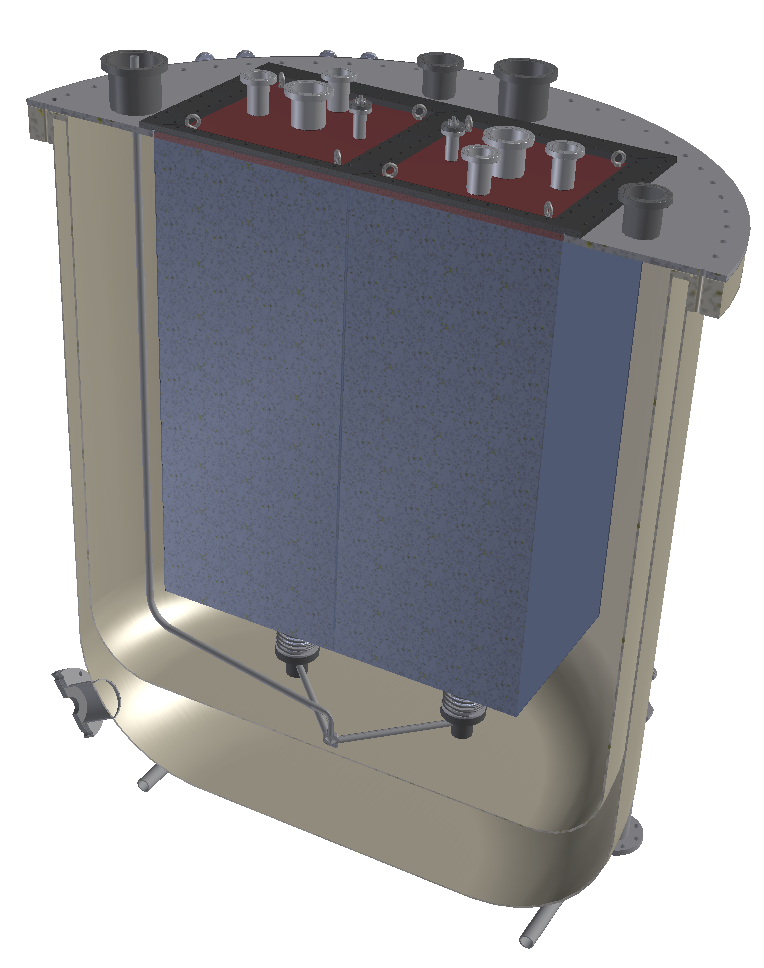
\includegraphics[width=0.5\textwidth]{plots/cutaway_cryostat}}
	\subfloat[Cutaway of a module]  {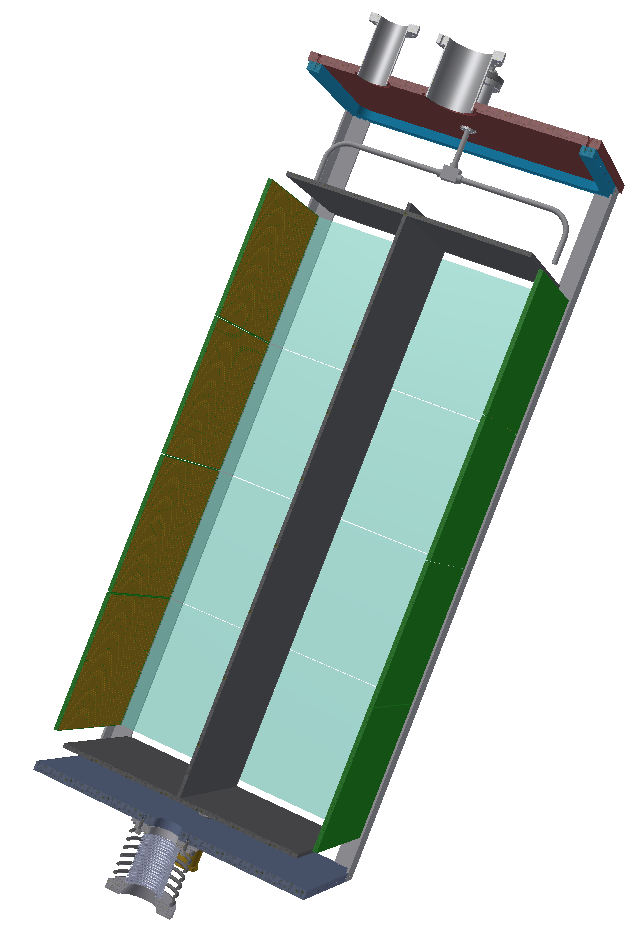
\includegraphics[width=0.45\textwidth]{plots/cutaway_module}}
	\caption[ArgonCube module cryogenic scheme]{In the cutaway of the cryostat the LAr exhaust connections are shown at the base of the modules, with the single line used to extract dirty argon for filtration and cooling (pump and filters not shown). The module cutaway shows the how the lines used to bring clean argon into the module at the top flange, where it is directed across the readout electronics to provide cooling.}
	\label{fig:cryo_scheme}
\end{figure}

ArgonCube offers true 3D tracking information using the LArPix cryogenic ASIC~\cite{larpix} pixelated charge readout. LArPix ASICs amplify and digitize the charge collected at single-pixel in the cold to mitigate the need for analogue signal multiplexing, thus produce unambiguous 3D information. 64 pixels can be connected to a single LArPix ASIC. The baseline design is for the 2x2 is a \SI{5}{\milli\metre} pixel pitch, corresponding to 40k pixels m$^{-2}$. Pixelated anode planes are located on the two module walls parallel to the cathode, each plane is \SI[product-units=repeat]{1.2x0.6}{\metre\squared}. The total area across all four modules is \SI{5.8}{\metre\squared}, which corresponds to 232k pixels. The readout electronics utilize two FPGA boards per module, connected to a single Ethernet switch. It should be noted that the pixel pitch may be reduced as prototypes develop, but this can be accommodated in the readout design. 

\begin{figure}[!ht]
	\centering
	\subfloat[ArCLight paddle] {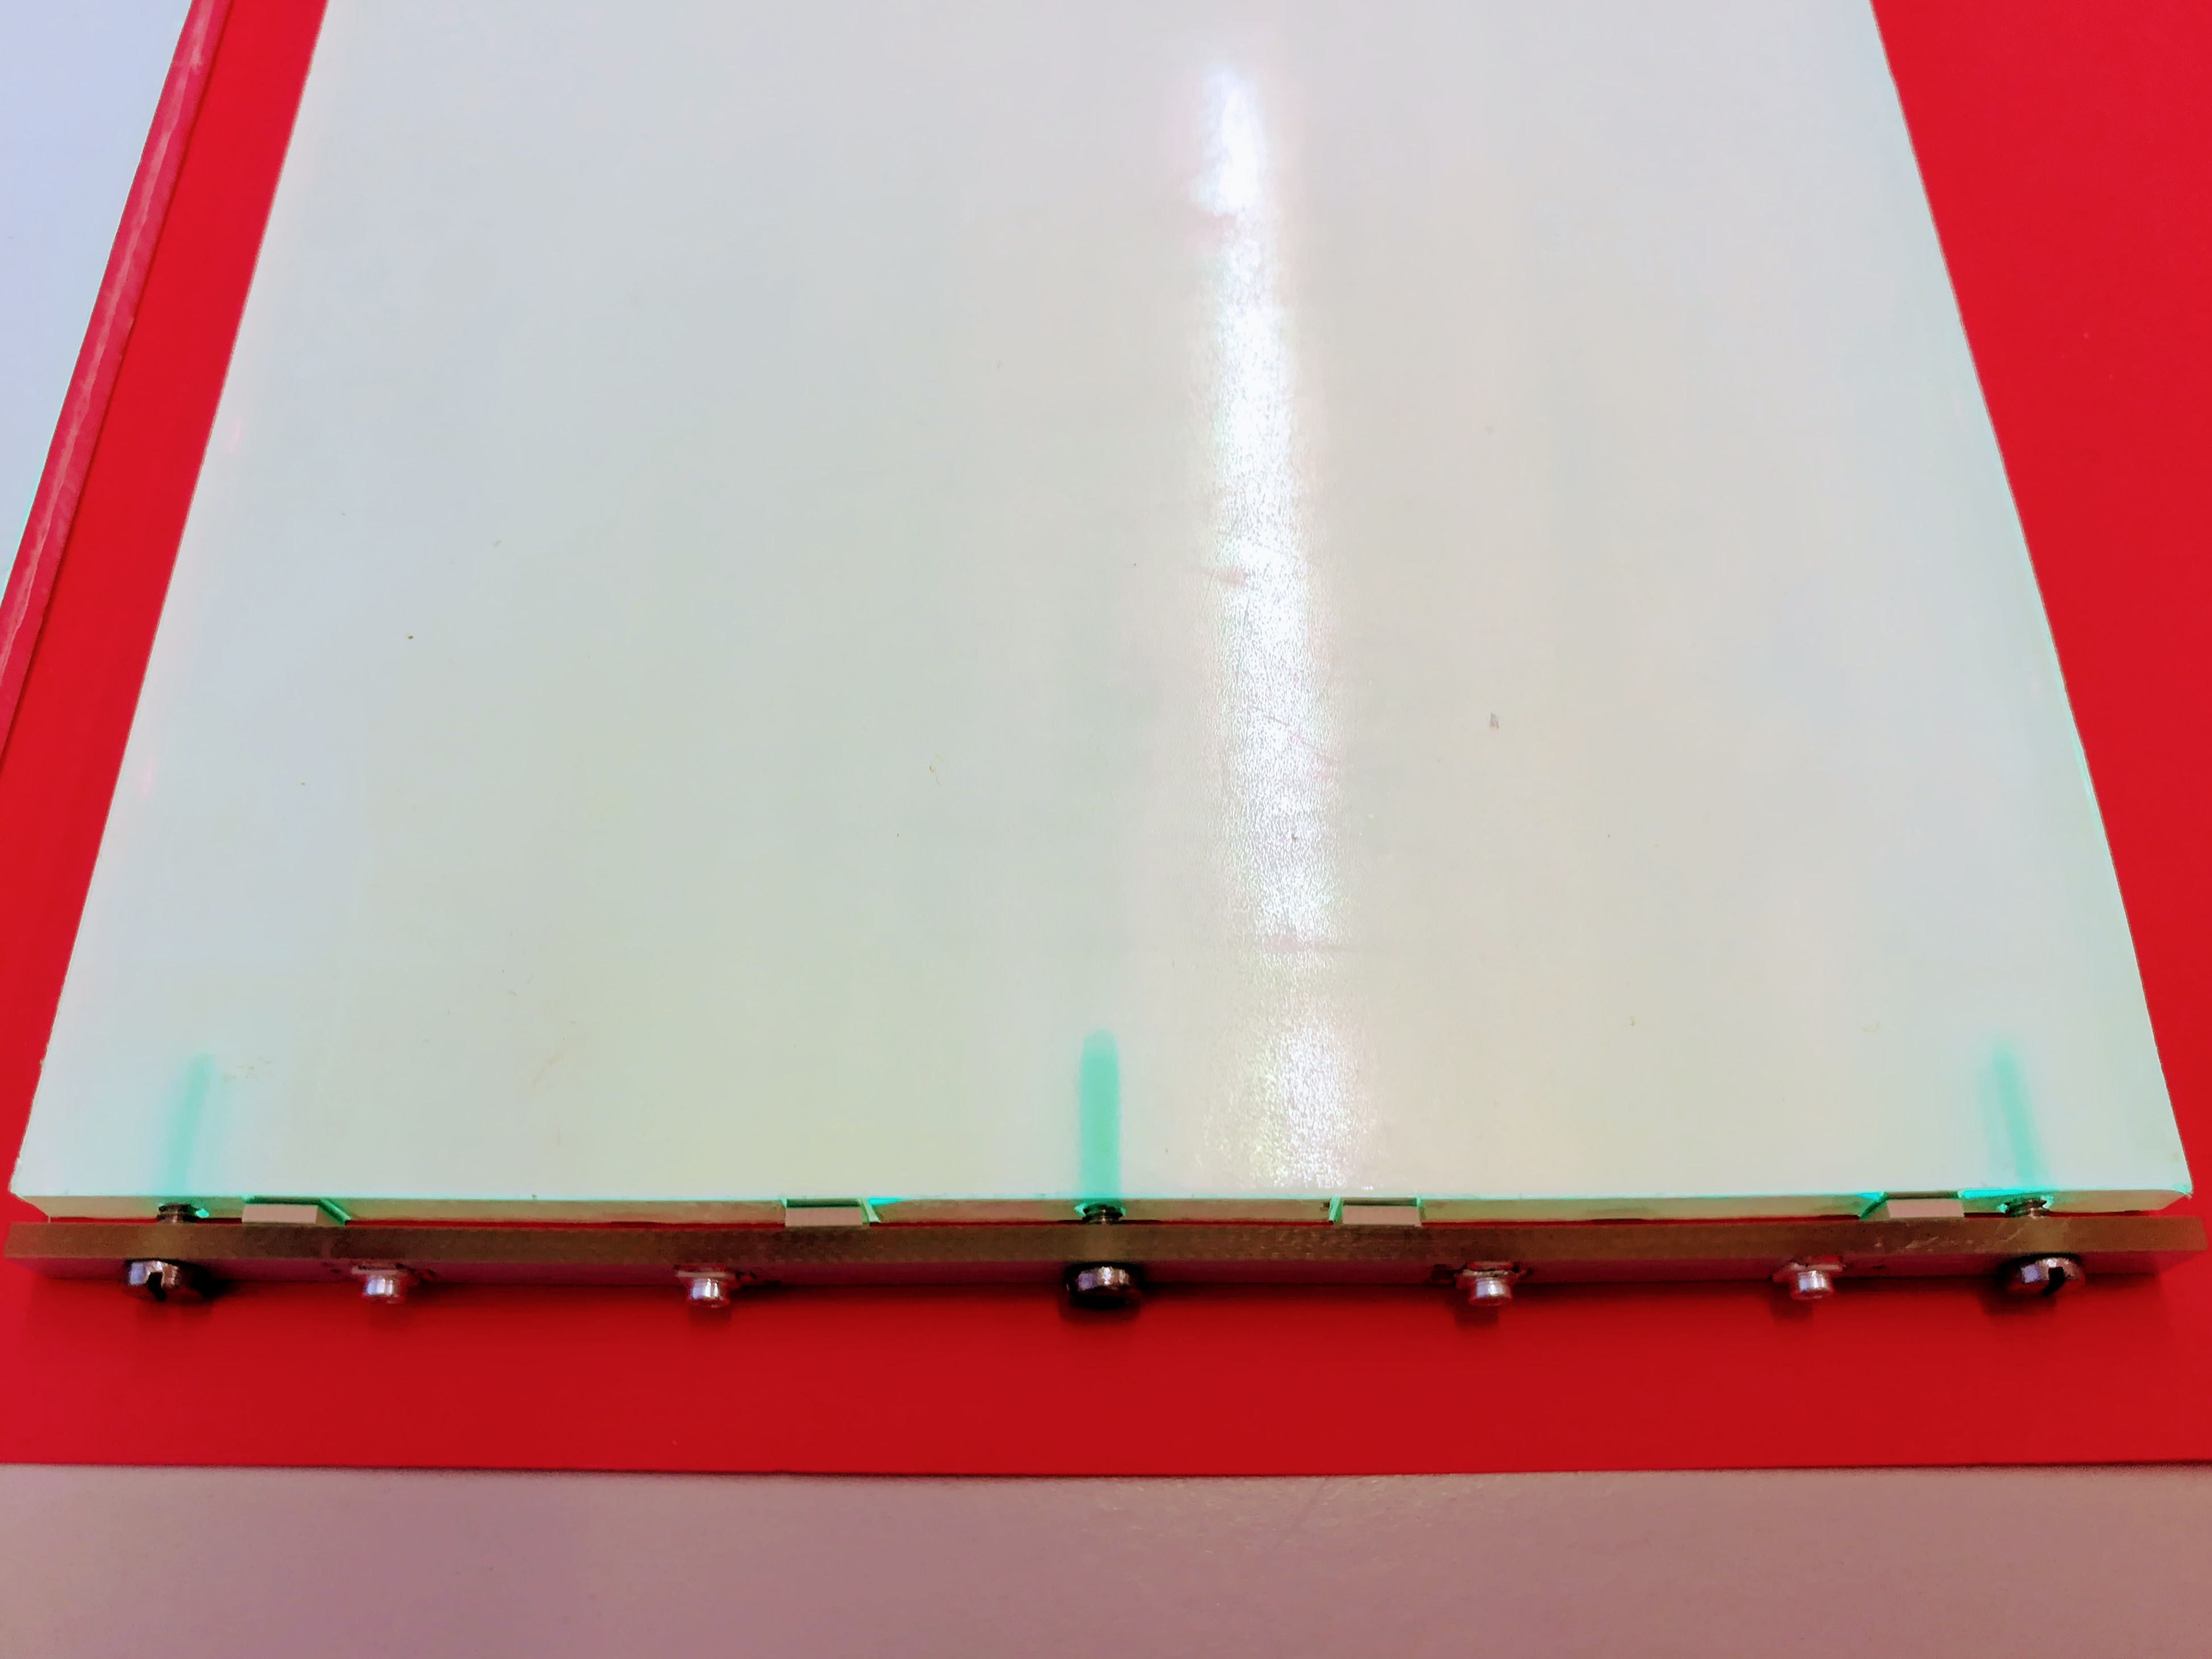
\includegraphics[width=0.454\textwidth]{plots/arclight}}
	\subfloat[ArCLight mounted on a pixel readout PCB]  {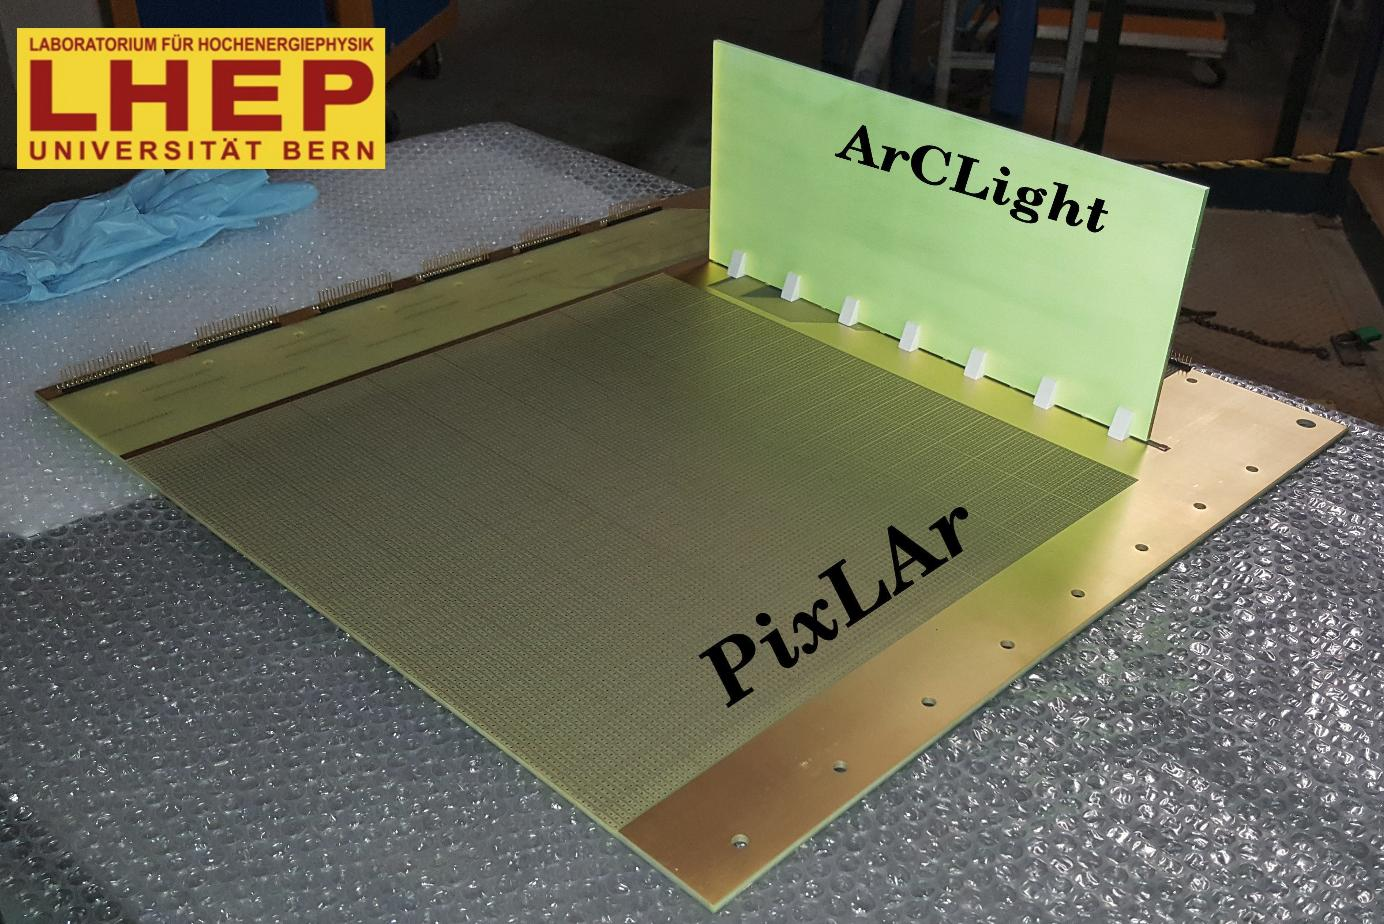
\includegraphics[width=0.51\textwidth]{plots/pixlar_arclight}}
	\caption{(a) A prototype ArgonCube light readout paddle built at the University of Bern. The paddle is 50~cm long and 10~cm wide, with four SiPMs coupled to one end. Reproduced from Ref.~\cite{argoncube_loi}. (b) ArClight paddle mounted on the PixLAr pixelated charge readout plane, as used in test beam studies at Fermilab.}
	\label{fig:arclight}
\end{figure}

The charge readout window (drift time) of \SI{137}{\micro\second} is long compared to the \SI{10}{\micro\second}~\cite{numi} beam spill length in the NuMI and LBNF beams.
For 1 MW beam intensity, the expected rate of neutrino interactions at the DUNE ND is roughly 0.5 per spill per ArgonCube module.  
With LArPix, reconstruction issues are greatly simplified compared to a projective readout TPC.
Tracks and connected energy deposits will frequently overlap in any 2D projection, but can be easily resolved with a full 3D readout.
However, disconnected energy deposits, such as those from photon conversions or neutron interactions in the detector, cannot be easily associated to a specific neutrino interaction.
This problem can be solved by incorporating fast timing information from the prompt scintillation light emitted in LAr.
The module's opaque cathode and walls contain scintillation light within each TPC (half module), improving the detection efficiency of the prompt component of the scintillation light. 
Furthermore, attenuation due to Rayleigh scattering, $6.6\times10^{-1}$~m in LAr~\cite{Rayleigh}, is mitigated by the maximum photon propagation lengths of only \SI{0.3}{\metre}. 
It is desirable to have a large area photon detection system to maximize the utility of scintillation light signals in the detector. 
To minimize any dead material within the active volume, it is also desirable that the light detection be as compact as possible. 
The solution pursued for the ArgonCube effort is ArCLight~\cite{arclight}, which is a very compact dielectric light trap that allows for light collection from a large area, inside high electric fields. 
An example ArCLight sheet is shown in Figure~\ref{fig:arclight}. These sheets are mounted on the walls of the module, inside the field shell, aligned with the drift direction, between the anode and the cathode. 
The additional \SI{5}{\milli\metre} deep dead volume is similar to the one caused by the charge readout in the perpendicular direction.

\subsubsection{Infrastructure for the 2x2 Demonstrator}
Infrastructure requirements in the MINOS ND hall are dominated by cryogenics, but power supply constraints should also be considered.
Control, slow monitoring and DAQ systems will be implemented before the detector arrives at Fermilab.  
A dedicated LN2 supply capable of \SI{0.75}{\litre\per\minute} is required for the constant cooling of the detector. 
A LAr supply is obviously also required, it will have to be determined if a closed-loop system is used in the hall, or provided from tanks on the surface.
Given the oxygen deficiency hazard (ODH) of LAr, dedicated exhaust and venting lines will be required, as well as a sump beneath the cryostat.
The sump will have to be accommodated into the platform used to align the detector with the beam.
The readout electronics will require a clean power supply, ideally separated for the utility supply used for the pumps and other detector components.       
The four modules each require a filtered High Voltage (HV) supply of \SI{30}{\kilo\volt}, which can be provided by a single external supply and a splitter, with the splitter serving as a low-pass filter for each TPC.
The DAQ will require a beam trigger and GPS timing inputs. 
The GPS is particularly important when reconstructing events across different detectors, as will be the case in DUNE ND.
A subsequent document will describe all infrastructure requirements in greater detail.

\subsection{Downstream tracking detectors}
\label{sec:tracking_detectors}
As well as an ArgonCube-like LAr component, the recommendations from the DUNE Near Detector Concept Study Group~\cite{dune_ndcsg} are for there to be additional, downstream tracking detectors in the DUNE ND to tag and measure the energies of particles which exit the downstream face of the LAr detector, and a magnetized component to identify the sign and measure the momentum of muons. It would therefore enhance the utility of ProtoDUNE-ND, as an intermediate-scale test of the DUNE ND, to include prototypes for these detectors, as many events in the high-energy NuMI ME beamline will not be fully contained in the ArgonCube 2x2 Demonstrator module (examples can be seen in Figures~\ref{fig:argonbox_event_display} and~\ref{fig:leaky_event}). 
Two downstream tracking options considered  by the DUNE Near Detector Concept Study Group are the Three Dimensional Scintillator Tracker (3DST), and the High-Pressure gaseous argon TPC (HPTPC).

The 3DST is a fully active plastic scintillator detector made of a large number of optically independent 1x1x1 cm$^{3}$ cubes read out in three orthogonal directions by wavelength shifting fibers~\cite{3dst}. The 3DST is envisioned as an upgrade to the plastic scintillator detectors read out in two dimensions used by T2K~\cite{t2k-fgd,t2k-ingrid}, NOvA~\cite{nova} and MINERvA~\cite{minerva-nim}, which will provide better angular coverage. Unfortunately, after consultation with the 3DST steering group, it was found that a large scale prototype suitable for ProtoDUNE-ND will not be available on the required timescale. If the situation changes, we note the desirability of including such a prototype in the proposed ProtoDUNE-ND effort.

The HPTPC is a high-pressure argon gas TPC which will operate inside a magnetic field~\cite{dune_ndcsg}. Its purpose is two-fold. Firstly, it acts as a downstream tracker for particles exiting the LAr detector, with a superior dE/dx resolution, and the ability to measure the sign and momentum of particles in the magnetic field. Secondly, it offers a lower threshold, higher resolution argon target detector than the LAr component. The HPTPC needs to be coupled with a ECal to detect escaping neutrals which will not convert in the argon gas, and to provide fast timing to differentiate tracks from multiple interactions. Although a HPTPC prototype is not ready at the time of writing this proposal, it is expected that a prototype will be produced during ProtoDUNE-ND operation, so the program should be flexible enough to incorporate a new detector component. 

As it is expected that the ProtoDUNE-ND setup may need to be reconfigured, with the addition of more components over time, and because DUNE-PRISM is now the baseline ND design, it is desirable to include a moveable cryogenic system for the ArgonCube 2x2 Demonstrator in ProtoDUNE-ND, which would allow the future moveable cryogenics for DUNE-PRISM to be tested.

